\section{Contexto y alcance}

Este trabajo representa la finalización del Grado de Ingeniería Informática, en el cual, se demostrarán algunas de las habilidades obtenidas a lo largo de los cursos, así como la capacidad de aprendizaje que se obtiene tras adquirir una amplía base de conocimientos.

La realización de CoWordle se centra en el aprendizaje por parte del autor de algunas tecnologías web, como la utilización de WebSockets como método de comunicación entre cliente y servidor.  Además, permite aprender también tecnologías como Docker, que permiten desplegar la aplicación de manera sencilla, independientemente del lugar de despliegue.

La tecnología de WebSockets es una tecnología que se estudia brevemente en el grado, pero no se llega a utilizar de manera práctica.

El objetivo de este trabajo es aprender a utilizar WebSockets, una tecnología que permite comunicar el cliente y el servidor de manera bidireccional, y que se utiliza en aplicaciones de tiempo real, como juegos online, aplicaciones de mensajería web o como base para otras tecnologías como WebRTC.

\textbf{CoWordle} es el juego web multijugador derivado de Wordle desarrollado para este trabajo. CoWordle añade a la versión original la capacidad de desafiar a otros jugadores y competir en tiempo real jugando una partida de Wordle simultánea.


\section{Wordle}

\textbf{Wordle} (Figura \ref{fig:wordle_app}) es un juego de navegador creado por el ingeniero Josh Wardle durante la pandemia de COVID-19. Desde el lanzamiento Wordle ha conseguido que millones de jugadores se conecten cada día para encontrar una palabra objetivo.

\begin{figure}
	\centering
	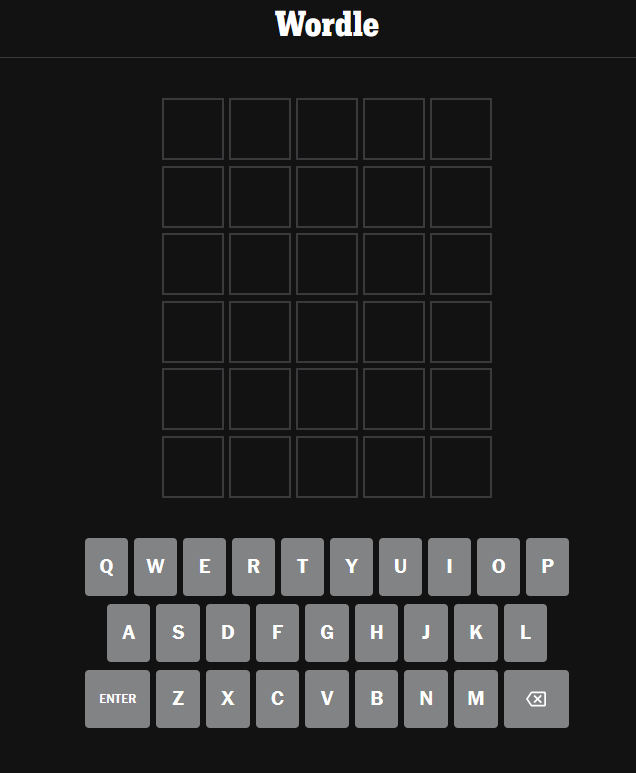
\includegraphics[clip=true, width=0.75\textwidth]{images/wordle.png}
	\caption{Aplicación oficial de Wordle.}
	\label{fig:wordle_app}
\end{figure}


\subsection{La historia de Wordle}

En sus comienzos Wordle solo era jugado por los amigos y familiares de Josh Wardle (Junio 2021), más tarde, Wardle publicó su juego en internet alcanzando menos de 100 jugadores durante las primeras semanas. Sin embargo, en enero de 2022 ya contaba con más de 300.000 jugadores cada día, y para finales de ese mismo mes ya jugaban millones de personas.

A finales de Enero de 2022, con la espectacular recepción del juego, The New York Times compró el juego por una cifra que no se ha publicado, pero que según el propio Wardle, ronda las 7 cifras.

En el informe de ganancias trimestrales de Marzo de 2022, The New York Times anunció que la compra de Wordle había traído a millones de jugadores a su página, y además muchos de estos nuevos jugadores, habían probado otros juegos ofrecidos por el noticiario.


\subsection{¿Comó se juega?}

Wordle es un juego en el que cada día, todos los jugadores del mundo tienen que descubrir la misma palabra.
Cada jugador tiene seis oportunidades para encontrar la palabra secreta, y cada oportunidad ofrece pistas sobre lo bien que has colocado cada letra del intento.

El juego utiliza colores como pistas para cada letra del intento:
\begin{itemize}
	\item El color gris indica que la letra no se encuentra en la palabra objetivo.
	\item El color naranja indica que la letra se encuentra en la palabra, pero no está en su posición correcta.
	\item El color verde indica que la letra se encuentra tanto en la palabra, como en la posición de la palabra correcta.
\end{itemize}

Cuando un jugador ha descubierto todas las letras de la palabra objetivo antes de quedarse sin intentos, el juego se termina y se muestra al jugador el resultado de la partida, mostrando entre otras estadísticas, el número de intentos requeridos.

Esta estadística ha sido uno de los grandes éxitos del juego, millones de jugadores intentan cada día conseguir la palabra en el menor número de intentos posibles, y comparan entre ellos los resultados con las integración de Facebook y Twitter de las que dispone la aplicación oficial.


\subsection{Otras aplicaciones derivados de Wordle}

Tras el éxito de Wordle, multitud de aplicaciones comenzaron a aparecer que clonaban las mismas mecánicas que Wordle, entre ellas, existen versiones en diferentes lenguajes o versiones donde tienes que resolver múltiples palabras simultáneamente como Octordle (Figura \ref{fig:octordle_app}) o Dordle (Figura \ref{fig:dordle_app}).


\begin{figure}
	\centering
	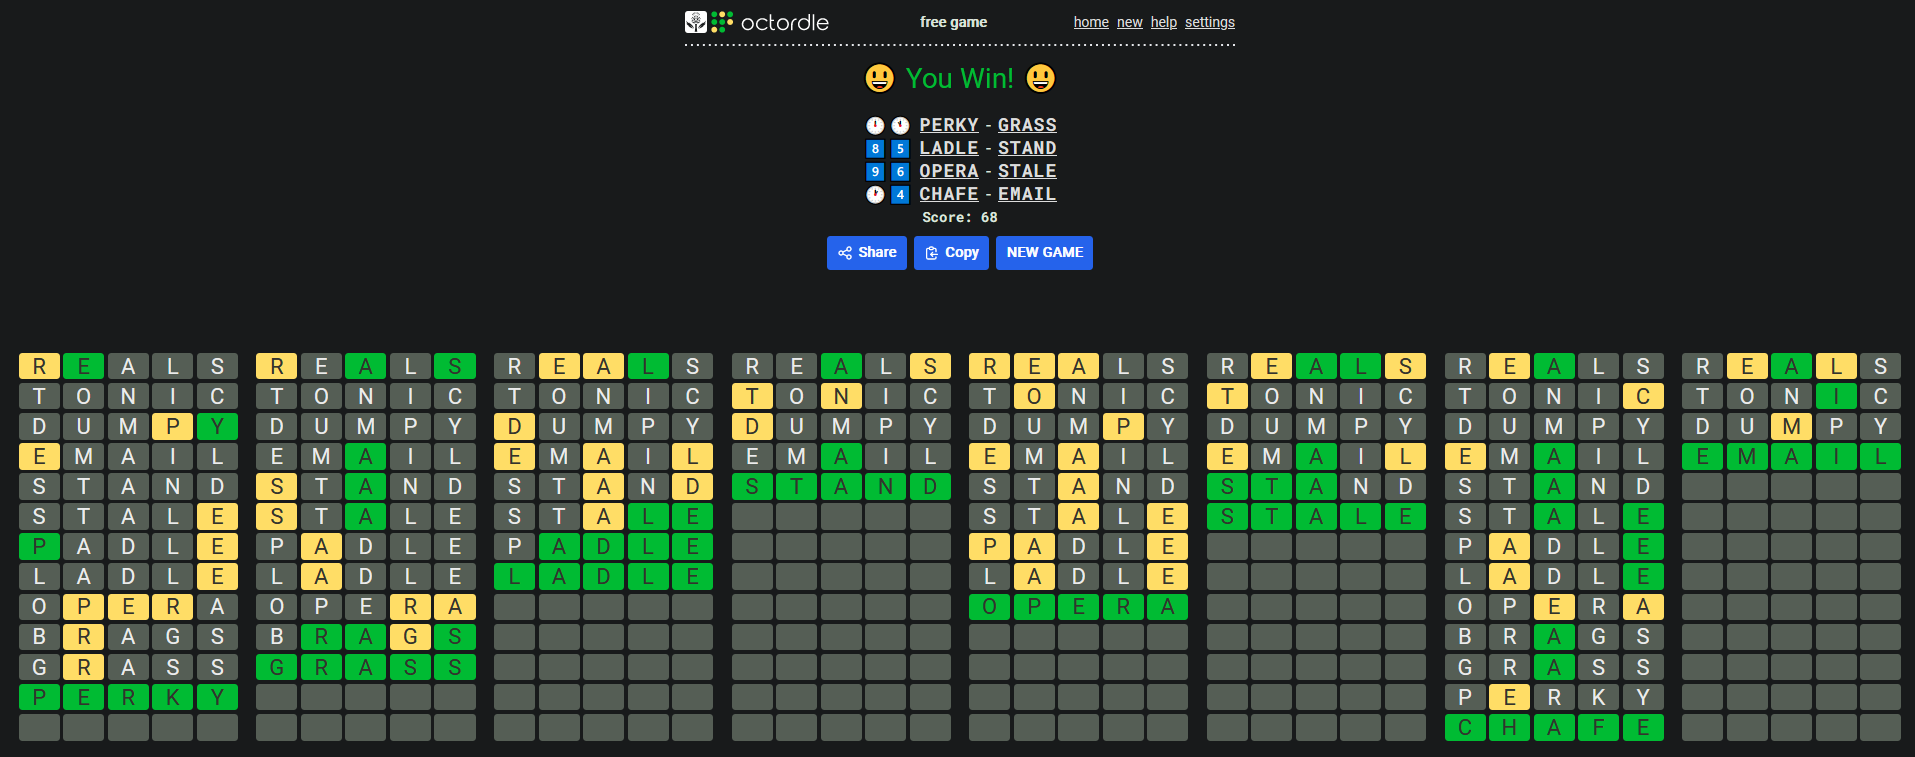
\includegraphics[clip=true,width=\textwidth]{images/octordle.png}
	\caption{Aplicación Octordle.}
	\label{fig:octordle_app}
\end{figure}

\begin{figure}
	\centering
	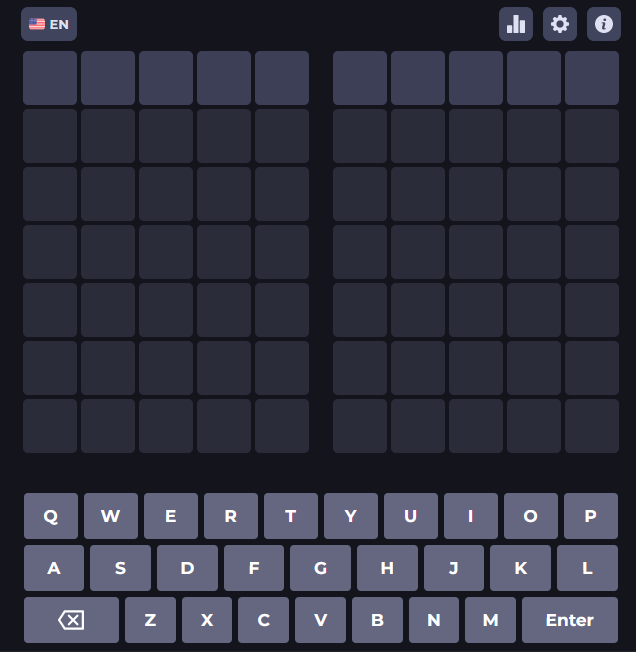
\includegraphics[clip=true,width=0.5\textwidth]{images/dordle.png}
	\caption{Aplicación Dordle.}
	\label{fig:dordle_app}
\end{figure}


A parte de inspirar multitud de juegos sobre palabras, existen variaciones como Globle, Worldle (Figura \ref{fig:worldle_app}), en las que el objetivo es descubrir países utilizando las formas de estos, o Numberle (Figura \ref{fig:numberle_app}), donde el objetivo el completar ecuaciones matemáticas.

\begin{figure}
	\centering
	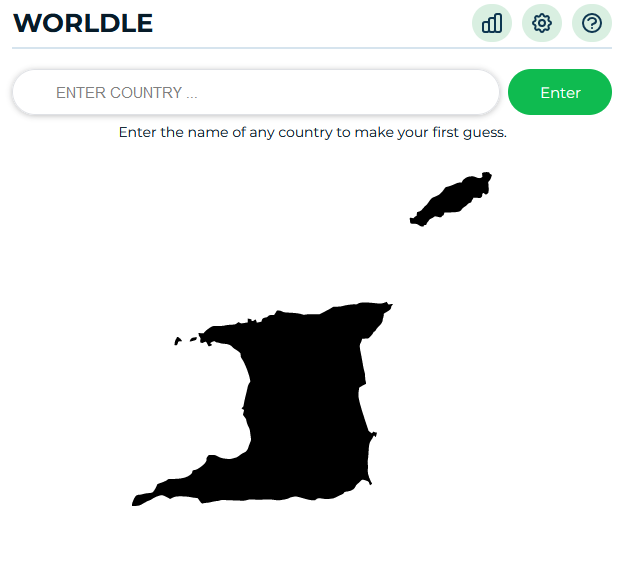
\includegraphics[clip=true,width=0.5\textwidth]{images/worldle.png}
	\caption{Aplicación Worldle.}
	\label{fig:worldle_app}
\end{figure}

\begin{figure}
	\centering
	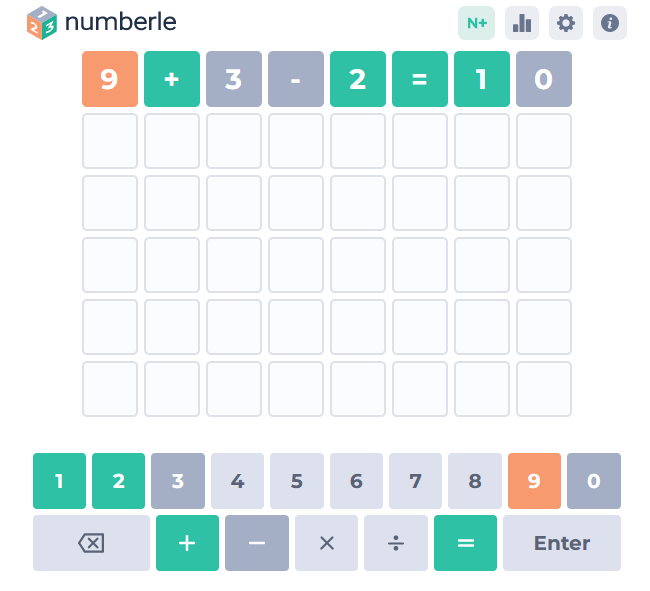
\includegraphics[clip=true,width=0.5\textwidth]{images/numberle.png}
	\caption{Aplicación Numberle.}
	\label{fig:numberle_app}
\end{figure}



\section{CoWordle}

CoWordle (Figura \ref{fig:cowordle_app}) añade otro \textit{twist} a Wordle, añadiendo un valor competitivo que aparece cuando múltiples jugadores tienen que descubrir la misma palabra en tiempo real. Los jugadores se encuentran con dos problemas simultáneos, el primero es conseguir averiguar la palabra antes de que se agoten todos los intentos, y el segundo es hacerlo antes que lo consigan los demás jugadores.

Para poder hacer que los jugadores compitan simultáneamente es necesario alguna tecnología que los permita comunicarse en tiempo real, por ello, CoWordle presenta una muy buena oportunidad para aprender sobre cómo funcionan y cómo se usan las tecnologías de tiempo real, aunque para la realización de este proyecto se ha utilizado únicamente WebSockets.

\begin{figure}
	\centering
	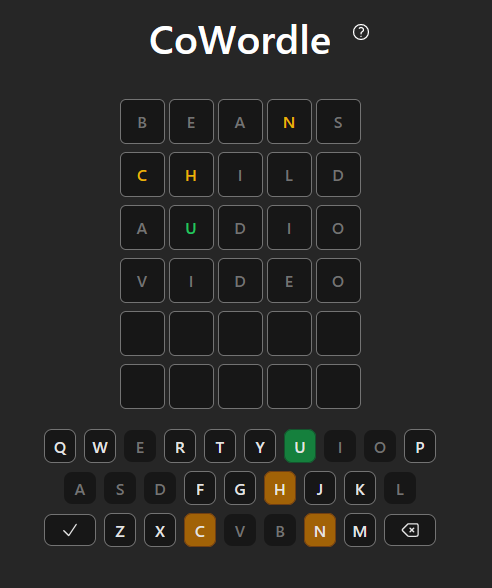
\includegraphics[clip=true, width=0.75\textwidth]{images/cowordle_app.png}
	\caption{Vista de juego CoWordle.}
	\label{fig:cowordle_app}
\end{figure}
